\chapter{Elliptische Kurven}
\label{kap:ek}

In diesem Abschnitt werden elliptische Kurven ad hoc eingeführt.
Teil des Datums einer elliptischen Kurve ist der Grundkörper $K$. Dies
ist a priori ein beliebiger Körper. Aber für uns sind die wichtigsten
Wahlen von Grundkörper die rationalen Zahlen $\IQ$, die reellen Zahlen
$\IR$ und die komplexen Zahlen $\IC$. Für Anwendungen in der
Kryptographie spielen  die endlichen Körper eine zentrale Rolle.

Es sei angemerkt, dass die Theorie elliptische Kurven im
arithmetischen Fall, d.h. für den $K=\IQ$ und verwandte Körper, ihre
volle Tiefe entfaltet. Falls der Grundkörper, so wie $\IC$,
algebraisch abgeschlossen ist, verschwinden viele arithmetische
Aspekte.

\section{Definition der elliptischen Kurve}

\begin{definition}
  Sei $K$ wie oben ein Körper.
  Eine \emph{Weierstrass-Gleichung}\index{Weierstrass-Gleichung} ist eine Gleichung vom Typ
  \begin{equation}
    \label{eq:weierstrass}
    E: Y^2 = X^3 + aX + b
  \end{equation}
  mit Unbekannten $X,Y$ und Koeffizienten $a,b\in K$, welche die
  Bedingung
  \begin{equation}
    \label{eq:disccondition}
    \Delta_E = -2^4(4a^3+27b^2)\not=0
  \end{equation}
  erfüllt. Wir bezeichnen $E$ auch als \emph{elliptische
    Kurve}\index{Elliptische Kurve}
  definiert über $K$.
  Die Grösse $\Delta_E$, ein Element aus $K$, heisst
  \emph{Diskriminante}\index{Diskriminante einer Weierstrass-Gleichung}
  der Weierstrass-Gleichung $E$. Zur Weierstrass-Gleichung $E$ gehört
  das \emph{Weierstrass-Polynom}\index{Weierstass-Polynom}\footnote{Diese Bezeichnung ist nicht
    Standard.} $Y^2- (X^3+aX+b)$.
\end{definition}

\begin{beispiele}\leavevmode
  \begin{enumerate}
  \item [(i)] In (\ref{eq:ellipticcong}) hatten wir die Gleichung $Y^2 = X^3-n^2X$
    für $n\in\IN$ betrachtet. Es handelt sich um eine
    Weierstrass-Gleichung $E_n$, für $K=\IQ$ (oder jeden Körper, der $\IQ$
    enthält) ist $\Delta_{E_n} = -2^4 3^3 n^4 \not=0$.
  \item[(ii)] Die Gleichung
    \begin{equation*}
      Y^2 = X^3,
    \end{equation*}
    definiert keine Weierstass-Gleichung, da (\ref{eq:disccondition})
    nicht erfüllt ist.
  \end{enumerate}
\end{beispiele}

\begin{bemerkung}
  Sei $K$ ein Körper der Charakteristik $2$, z.B. $K=\IF_2$, und
  $a,b\in K$. Dann ist $Y^2 = X^3+aX+b$ keine Weierstrass-Gleichung,
  da (\ref{eq:disccondition}) nicht erfüllt ist. In $K$ gilt $1+1=0$.

  Das ist etwas unbefriedigend, da für Anwendung in der Kryptographie
  endliche Körper der Charakteristik $2$ wichtig sind. Weiterhin ist es
  auch theoretischer Sicht wichtig, einen sinnvollen Begriff von
  elliptischen Kurven über alle Körper
  zu haben. Um Charakteristik $2$ (und auch $3$) abzudecken, muss man
  die Definition von Weierstrass-Gleichung verallgemeinern. Wir werden
  dies hier nicht tun, da es etwas technisch ist. Kurzum reicht es mit
  den sogenannten langen Weierstrass-Gleichungen vom Typ
  \begin{equation*}
    Y^2 + a_1 XY + a_3 Y = X^3+a_2 X^2 + a_4 X + a_6
  \end{equation*}
  mit entsprechender (aber kompliziertere) Diskriminanten-Bedingung
  \begin{alignat*}1
    &-a_6 a_1^6 + a_4 a_3 a_1^5 + ((-a_3^2 - 12 a_6) a_2 + a_4^2) a_1^4 +
    (8 a_4 a_3 a_2 + (a_3^3 + 36 a_6 a_3)) a_1^3\\
    &+ ((-8 a_3^2 - 48 a_6) a_2^2 +
    8 a_4^2 a_2 +
    (-30 a_4 a_3^2 + 72 a_6 a_4)) a_1^2 \\
    &+ (16 a_4 a_3 a_2^2 +
    (36 a_3^3 + 144 a_6 a_3) a_2 - 96 a_4^2 a_3) a_1 \\
    &+ ((-16 a_3^2 -
    64 a_6) a_2^3 + 16 a_4^2 a_2^2 + (72 a_4 a_3^2 + 288 a_6 a_4) a_2
    \\
    & +
    (-27 a_3^4 - 216 a_6 a_3^2 + (-64 a_4^3 - 432 a_6^2))) \not=0.
  \end{alignat*}
  zu arbeiten.

  In Charakteristik $\not=2$ und $\not=3$ kann man jede lange
  Weierstrass-Gleichung mittels quadratisch und kubischem Ergänzen
  durch eine affine lineare Transformation auf eine
  Weierstrass-Gleichung umformen. 
\end{bemerkung}

Nun wollen wir die Bedingung (\ref{eq:disccondition}) rechtfertigen.
Die partiell Ableitung eines Polynoms ist formal über jedem Körper
definiert, es ist kein Grenzwertbegriff notwendig.

\begin{lemma}
  \label{lem:smooth}
  Sei $F$ das Weierstrass-Polynom einer Weierstrass-Gleichung
  (\ref{eq:weierstrass}). Sei $(x,y)\in K^2$ mit $F(x,y)=0$. Dann
  gilt
  \begin{equation*}
    \frac{\partial F}{\partial X}(x,y)\not=0 \qoq
    \frac{\partial F}{\partial Y}(x,y)\not=0.
  \end{equation*}
\end{lemma}
\begin{proof}
  Es gilt $F = Y^2 - X^3-aX-b$ und $-2^4(4a^3+27b^2)\not=0$.
  Insbesondere gilt $2\not=0$ in $K$. Weiterhin
  \begin{equation*}
    \frac{\partial F}{\partial Y} = 2Y. 
  \end{equation*}

  Sicher ist diese Ableitung $\not=0$ an jedem Punkt $(x,y)$ mit
  $y\not=0$.
  Es reicht also zu zeigen, dass $    \frac{\partial F}{\partial
    X}(x,0)\not=0$, falls $F(x,0)=0$.

  Nun gilt
  \begin{equation*}
    \underbrace{(X^3+aX+b)}_{=-F(X,0)}(288aX-432b) +
    \underbrace{(-3X^2-a)}_{= -\partial F/\partial X}(96aX^2 - 144bX + 64a^2)
    = -2^4(4a^3+27b^2) =\Delta_E\not= 0
  \end{equation*}
  nach Voraussetzung.
  Wir substituieren $X$ durch $x$ und finden 
  $\frac{\partial F}{\partial
    X}(x,0)\not=0$ da $F(x,0)=0$.  
\end{proof}

\begin{bemerkung}
  \label{bem:tangente}
  Im Fall $K=\IR$ können wir dieses letzte Lemma geometrisch wie folgt
  interpretieren.
  Sei $(x,y)\in\IR^2$ eine Nullstelle von $F$, dem Weierstrass-Polynom
  einer Weierstrass-Gleichung. Wir setzen
  $$\alpha = -\frac{\partial F}{\partial Y}(x,y) \quq
  \beta = \frac{\partial F}{\partial X}(x,y).$$
  Dann ist $(\alpha,\beta)$ nicht der Nullvektor.

  Aus dem Satz von der impliziten Funktion folgt, dass wir die
  Nullstellenmenge von $F$ in $\IR^2$ in der Nähe von $(x,y)$ durch
  den Graph einer glatten Funktion (nach einem möglichen Koordinatentausch)
  ausdrücken können. 

  Weiterhin ist die Menge
  \begin{equation*}
    T = \{(x+\alpha t,y+\beta t) : t\in\IR\}
  \end{equation*}
  eine Gerade durch $(x,y)$. Wir definieren $f(t) =
  F(x+t\alpha,y+t\beta)$ für alle $t\in\IR$. 
  Dann gilt 
  \begin{equation*}
    \frac{d\gamma}{dt}(t)
    = \underbrace{F(x,y)}_{=0} + \left(\underbrace{\alpha \frac{\partial F}{\partial X}(x,y)
    +\beta \frac{\partial F}{\partial Y}(x,y)}_{=0}\right)t + \text{(Terme der
      Ordnung $\ge 2$ in $t$)}.
  \end{equation*}
  
  Also hat $t\mapsto F(x+t\alpha,y+t\beta)$ eine mehrfache Nullstelle
  bei $t=0$. Dies bedeutet, dass $T$ die Tangente an der
  Nullstellenmenge von $F$ ist.

  Zusammengefasst: die Gerade durch $(x,y)$ mit Richtungsvektor
  \begin{equation*}
    \left(-\frac{\partial F}{\partial Y}(x,y),\frac{\partial F}{\partial X}(x,y)\right)
  \end{equation*}
  liegt tangential an der Nullstellenmenge von $F$.
\end{bemerkung}

Die Schlussfolgerung von Lemma~\ref{lem:smooth} besagt, dass die
Nullstellenmenge einer Weierstrass-Gleichung an jedem Punkt einer
Bedingung genügt, welche sich zumindest im reellen Fall
als ``Glattheitsbedingung'' verstehen lässt.

\begin{definition}
  \label{def:tangentensteigung}
  Sei $F$ das Weierstrass-Polynom einer Weierstrass-Gleichung. Falls
  $(x,y)\in K$ und $F(x,y)=0$ mit  $y\not=0$, dann heisst
  \begin{equation*}
    \frac{\frac{\partial F}{\partial X}}{-\frac{\partial F}{\partial
        Y}}(x,y) = \frac{3x^2+a}{2y}
  \end{equation*}
  \emph{Tangentensteigung} an $(x,y)$. 
\end{definition}

Sei $m$ die Tangentensteigung an $(x,y)$.
So wie in Beispiel \ref{bem:tangente} zeigt man, dass
$F(x+t,y+mt)$ bei $t=0$ eine Nullstelle der Ordnung $\ge 2$ hat. 

\begin{beispiel}
  Die Lösungsmenge von $Y^2=X^3$ hat bei $(0,0)$ eine ``Spitze''.  Die
  Nullstellenmenge ist an diesem Punkt nicht glatt, vgl.
  Abbildung~\ref{fig:cusp} links.

  \begin{figure}
    \centering    
    \caption{Lösungsmenge von $Y^2=X^3$ (links) und $Y^2 = X^3-X$ (rechts)}
    \label{fig:cusp}
    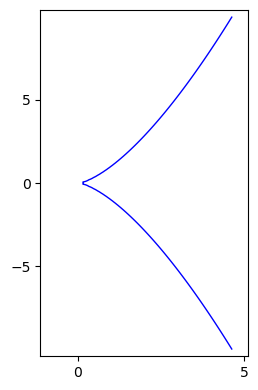
\includegraphics[width=0.3\textwidth]{./plots/cusp.png}
    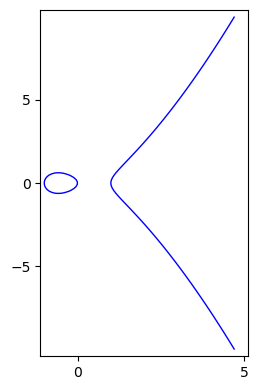
\includegraphics[width=0.3\textwidth]{./plots/smooth_n_equal_1.png}
  \end{figure}

  In der gleichen Abbildung rechts ist eine glatte Kurve zu sehen.
\end{beispiel}

\section{Das Gruppengesetz}

In diesem Abschnitt werden wir zeigen, wie man auf der Lösungsmenge
einer Weierstrass-Gleichung zusammen mit einem zusätzlichen Punkt,
eine Gruppenstruktur definieren kann. Die Konstruktion kann man rein
geometrisch veranschaulichen. Wie oben bezeichnet $K$ ein Körper in dem
sich alles abspielt (sofern nicht anders vermerkt). 

\begin{definition}
  Sei $Y^2 = X^3+aX+b$ eine Weierstrass-Gleichung $E$.
  Wir definieren 
  \begin{equation*}
    E(K) = \{(x,y) \in K^2 : y^2 = x^3 + ax+b\} \cup \{\cO\}.
  \end{equation*}
  wobei $\cO$ zunächst ein weiteres Element ist, welches nicht in
  $K^2$ liegt. Man nennt $E(K)$ die \emph{Menge der $K$-rationalen Punkten
  von $E$}. 
\end{definition}

\begin{beispiel}
  \label{bsp:fermat}
  Für die Weierstrass-Gleichung $E$ gegeben durch $Y^2 = X^3-X$ und
  für $K=\IQ$ besagt der 
  Satz von Fermat, Satz~\ref{satz:fermat2}, dass
  $$ E(\IQ) = \{(0,0), (\pm 1,0), \cO\} .$$
  aus vier Elementen besteht. 
\end{beispiel}


\begin{beispiel} Sei $E: Y^2-(X^3+aX+b)$ eine Weierstrass-Gleichung
  mit $a,b$ Elemente eines Körpers $K$.
  \begin{enumerate}
  \item [(i)]  Für $K=\IR$ und für  
    alle hinreichend grosse 
  $x\in\IR$ gibt es $y\in\IR$ mit $y^2 = x^3+ax+b$. Folglich ist $E(\IR)$ stets
  überabzählbar unendlich.  
  \item[(ii)] Für $K=\IC$ und für alle $x\in\IC$ gibt es $y\in\IC$ mit
    $y^2 = x^3+ax+b$. Dabei verwenden wir, dass jede komplexe Zahl
    eine komplexe Quadratwurzel besitzt (oder dass $\IC$ algebraisch
    abgeschlossen ist). Also ist $E(\IC)$
    überabzählbar unendlich.  
  \end{enumerate}
\end{beispiel}

Wir werden zeigen, dass wir $E(K)$ mit der Struktur einer abelschen
Gruppe verstehen können. Dazu müssen wir
\begin{itemize}
\item eine Verknüpfung $E(K)\times E(K)\rightarrow E(K)$,
\item eine Inversionsabbildung $E(K)\rightarrow E(K)$,
\item sowie ein neutrales Element in $E(K)$
  definieren.
\end{itemize}
Danach muss man überprüfen, dass alle Bedingungen der Definition einer abelschen Gruppe
erfüllt sind.
  
\subsection{Die Verknüpfung}
\label{sec:verknuepfung}

Sei $E$ eine Weierstrass-Gleichung gegeben durch $Y^2 = X^3+aX+b$ mit
$a,b\in K$. 
In einem ersten Schritt werden wir eine Verknüpfung
\begin{equation*}
  + \colon E(K)\times E(K) \rightarrow E(K)
\end{equation*}
definieren. Es ist üblich, die Verknüpfung mit ``$+$'' zu bezeichnen.
% Später werden wir feststellen, dass die so konstruierte Gruppe eine
% abelsche Gruppe ist. 

Seien $P$ und $Q$ Elemente von $E(K)$. Wir werden bereits in der
Konstruktion überprüfen, dass die Verknüpfung $+$ die Bedingung
$$
P+Q=Q+P\quad\text{für alle}\quad P,Q\in E(K)
$$
erfüllt. Hieraus werden wir folgern, dass die Gruppe $E(K)$ abelsch
ist.

Es folgt eine Aufspaltung in verschiedene Fälle.

\medskip
\textbf{Fall 1: Die Menge $\{P,Q,\cO\}$ hat drei Elemente.} In diesem
Fall gilt $P = (x_1,y_1)$ und $Q = (x_2,y_2)$. Weiterhin haben wir
$P\not=Q$.
Daher gibt es genau eine Gerade $G$ durch $P$ und $Q$.

Wir unterscheiden zwei Unterfälle. 

\textbf{Unterfall 1a. Es gilt $x_1\not=x_2$.} In diesem Fall hat die
Gerade $G$ (endliche) Steigung $m = \frac{y_2-y_1}{x_2-x_1}\in K$. In
anderen Worten, sie lässt sich durch die Abszisse parametrisieren
\begin{equation*}
  G = \{(x,mx+q) : x\in K \}
\end{equation*}
wobei $q=y_1-m x_1$. Vgl. Abbildung \ref{fig:unterfall1a} darin ist $G$
gestrichelt.

\begin{figure}[h]
  \centering    
  \caption{$E: Y^2 = X^3-5^2 X,P = (-4,6),Q = (\frac{1681}{144},-\frac{62279}{1728})$}
  \label{fig:unterfall1a}
  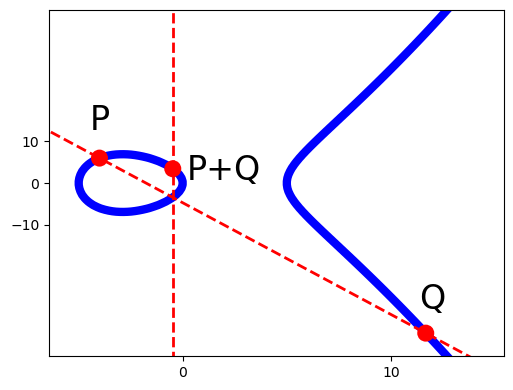
\includegraphics[width=0.3\textwidth]{./plots/unterfall1a.png}
\end{figure}
 
Daher sind $P$ und $Q$ Schnittpunkte der Gerade $G$ mit der Menge
$E(K)\ssm \{\cO\}$. Mit Vielfachheiten gezählt hat die Gerade $G$
jedoch drei Schnittpunkte mit der Lösungsmenge von $Y^2=X^3+aX+b$. Wir
können dies wie folgt direkt überprüfen. Dazu definieren wir
das Polynom
\begin{equation*}
  A = (mX+q)^2 - (X^3+aX+b) =-X^3+m^2X +\text{(Terme von Grad $\le 1$ in $X$)}
  \in K[X]. 
\end{equation*}

Das Polynom $A$ hat Grad $3$  und wir kennen bereits zwei verschiedene
Nullstellen: $x_1,x_2\in K$. Daher lässt sich $A$ durch $X-x_1$ und
$X-x_2$ teilen. Es gilt also $A = -(X-x_1)(X-x_2)(X-x_3)$, dabei muss
$x_3$ als wiederum ein Element in $K$ sein, denn es gilt $x_1+x_2+x_3
= m^2$, also
\begin{equation*}
  x_3 = \left(\frac{y_2-y_1}{x_2-x_1}\right)^2-x_2-x_1.
\end{equation*}
Nach Konstruktion ist das Paar $(x_3,y_3)$ mit  $y_3=mx_3+q$ eine
Nullstelle von $Y^2-(X^3+aX+b)$. Weiterhin ist auch $(x_3,-y_3)$ eine
Nullstelle.

In Unterfall 1a definieren wir
\begin{equation*}
  P+Q = (x_3,-y_3) \in E(K)\ssm \{\cO\}.
\end{equation*}

Sind wir in  Unterfall 1a, so ist auch das Paar $(Q,P)$ in Unterfall
1a. Es gilt $P+Q=Q+P$, da die Gerade und sowohl $(m,q)$ unabhängig von
der Reihenfolge von $P,Q$ ist. 

\textbf{Unterfall 1b. Es gilt $x_1=x_2$.} Nun liegt die Gerade $G$
senkrecht zur Abszisse, vgl. Abbildung~\ref{fig:unterfall1b}. Es gilt
\begin{equation*}
  y_1^2 = x_1^3+a x_1 +b = x_2^3+a x_2 +b = y_2^2
\end{equation*}
und daher $y_1=-y_2$ da $P\not=Q$. Nun stehen wir vor einem
Dilemma, die Gerade $G$ hat keine weiteren Schnittpunkte mit $E(K)$ in
der Ebene $K^2$. Jetzt kommt uns der Punkt $\cO$ zur Hilfe.

In Unterfall 1b definieren wir
\begin{equation*}
  P+Q = \cO \in E(K).
\end{equation*}

Vertauscht man $P,Q$ so bleiben wir in Unterfall 1b und es gilt
trivialerweise $P+Q=Q+P$.  

\begin{figure}
  \centering    
  \caption{$E: Y^2 = X^3-5^2 X,P = (-4,6),Q = (-4,-6)$}
  \label{fig:unterfall1b}
  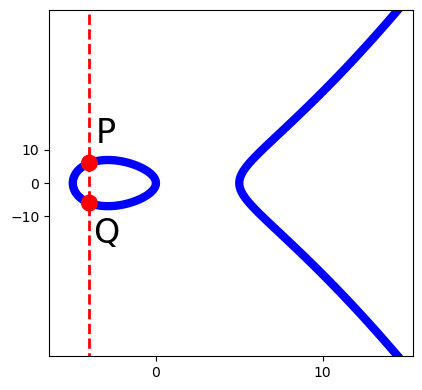
\includegraphics[width=0.3\textwidth]{./plots/unterfall1b.png}
\end{figure}

\medskip
\textbf{Fall 2: Die Menge $\{P,Q,\cO\}$ hat zwei Elemente.} Auch hier
gibt es mehrere Unterfälle.

\textbf{Unterfall 2a: Es gilt $P=Q\not=\cO$ und $P=(x,y)$ mit $y\not=0$.}
%Wir schreiben $P=Q=(x,y)$ mit $x,y\in K$.

Die Gerade, welche in Fall 1 konstruiert wurde, ist nun nicht
eindeutig bestimmt.

Etwas Intuition schafft die folgende Überlegung. Wir
versetzen uns in die reelle Welt und ersetzen den Punkte $Q$ durch
eine Folge von Punkten $(Q_n)_{n\in\IN}$ aus $E(\IR)\ssm\{Q,\cO\}$, dessen
Koordinaten für $n\rightarrow\infty$ gegen $Q=P$ konvergieren.
Die Gerade $G_n$ durch $P$ und $Q_n$ ist wohldefiniert und die Summe
$P+Q_n$ lässt sich mit der Vorschrift aus Fall 1 bestimmen.
Anschaulich nähert sich die Gerade $G_n$ der Tangente an
$E(\IR)\ssm\{\cO\}$ durch den Punkte $P$. Vgl.
Abbildung~\ref{fig:unterfall2a}. 

\begin{figure}
  \centering    
  \caption{$E: Y^2 = X^3-5^2 X,P = Q=(-4,6)$}
  \label{fig:unterfall2a}
  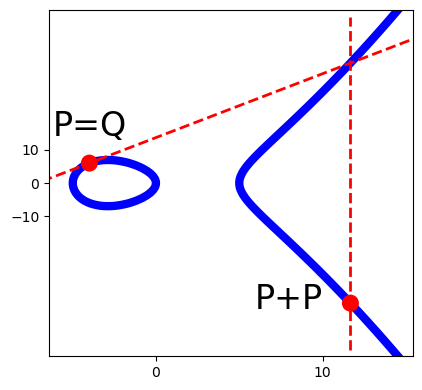
\includegraphics[width=0.3\textwidth]{./plots/unterfall2a.png}
\end{figure}

Für einen allgemeinen Körper können wir zwar nicht mit
Grenzwertbegriffen argumentieren, aber wir haben
dank Bemerkung~\ref{bem:tangente} und Definition
\ref{def:tangentensteigung} eine algebraische Version der Tangente
gefunden.


Für $y\not=0$ dürfen wir  Definition \ref{def:tangentensteigung}
anwenden. Das weitere Vorgehen ist vergleichbar mit Unterfall 1a.
Wir setzen
$$m =  \frac{3x^2+a}{2y}\in K\quq q = y-mx\in K.$$
Das Polynom
$$
A = (mX+a)^2 - (X^3+aX+b) \in K[X]
$$
hat  eine Nullstelle der Ordnung $\ge 2$ in $x$. Dies lässt sich
rein formal mit Hilfe der Definition von $m$ überprüfen.
Also gilt $A = -(X-x)^2(X-x')$ für ein $x'\in K$. Dabei gilt
\begin{equation*}
  x' = m^2 - 2x = \left(\frac{3x^2+a}{2y}\right)^2 - 2x. 
\end{equation*}

Der Punkt $(x',y')$ mit $y'=mx'+q$ liegt in $E(K)$. Wie in Unterfall
1a liegt $(x',-y')$ auch in $E(K)$. 
In Unterfall 2a
definieren wir
\begin{equation*}
  P+Q = P+P = \left(x',-y'\right).
\end{equation*}

Trivialerweise gilt $P+Q=Q+P$ in diesem Unterfall.

\textbf{Unterfall 2b: Es gilt $P=Q\not=\cO$ und $P=(x,0)$.}
Im Fall $y=0$ ist die Tangente durch $P$ and $E(K)$ parallel zur
Ordinate. Wir 
definieren
\begin{equation*}
  P+Q = P+P = (x,0)+(x,0) = \cO. 
\end{equation*}
Trivialerweise gilt $P+Q=Q+P$ in diesem Unterfall.

\textbf{Unterfall 2c: Es gilt $P=\cO\not=Q$.}
Wir definieren 
\begin{equation*}
  P+Q = \cO + Q = Q. 
\end{equation*}


\textbf{Unterfall 2d: Es gilt $P\not=\cO=Q$.}
Dieser Fall ist analog zu Unterfall 2b, wir definieren hier
\begin{equation*}
  P+Q = P+\cO = P. 
\end{equation*}
Vergleicht man Unterfälle 2b und 2c, so sehen wir $P+Q=Q+P$, falls
$P=\cO$ oder $Q=\cO$. 


\medskip
\textbf{Fall 3: Die Menge $\{P,Q,\cO\}$ hat ein Elemente.} Es gilt
$P=Q=\cO$ und wir definieren
\begin{equation*}
  P+Q = \cO+\cO = \cO. 
\end{equation*}
Trivialerweise gilt $P+Q=Q+P$. 

\subsection{Die Inversionsabbildung}

Sei $P\in E(K)$. Hier gibt es nur zwei Fälle.

\textbf{Fall 1. Es gilt $P\not=\cO$.} In diesem Fall ist $P=(x,y)$.
Wegen $y^2 = x^3+ax+b$ ist auch $(x,-y)$ eine Lösung der Weierstrass-Gleichung.
Wir  definieren
$$
-P = (x,-y)\in E(K)\ssm\{\c0\}.
$$

\textbf{Fall 2. Es gilt $P=\cO$.} 
Wir  definieren
$$
-P = \cO \in E(K).
$$

\subsection{Das neutral Element}
Es sollte nun nicht überraschen, dass wir $\cO$ als das neutrale
Element designieren.

\section{Überprüfung der Gruppenaxiome}

\begin{satz}
  Sei $E$ eine Weierstrass-Gleichung mit Koeffizienten in einen Körper
  $K$. Sei $+$ die Verknüpfung auf $E(K)$ aus
  Abschnitt~\ref{sec:verknuepfung}.
  Das Tripel $(E(K),\cO,+)$ ist eine abelsche Gruppe. 
\end{satz}

Die Abbildung $+\colon E(K)\times E(K) \rightarrow E(K)$ ist
wohldefiniert. Seien $P,Q\in E(K)$ beliebig.
Wir haben bereits überprüft, dass $P+Q=Q+P$. Also ist
$(E(K),\cO,+)$  eine abelsche Gruppe, sofern es eine Gruppe ist. 
Weiterhin überprüfen wir mit der Hilfe von den  Unterfällen
1b, 2b und Fall 3 der Konstruktion, dass
$$  (-P)+P = \cO$$
für alle $P\in E(K)$ gilt.

Weiterhin ist $\cO + P = P $ für alle $P\in \cO$, dies folgt aus den
Unterfällen 2c, 2d und Fall 3 in der Konstruktion. 

Schliesslich muss noch die Assoziativität der Verknüpfung gezeigt
werden. Dies läuft auf die Gleichung
$$
P + (Q + R) = (P+Q)+R$$
für alle $P,Q,R\in E(K)$ hinaus.

Das ist ein nicht-trivialer Schritt den wir hier nicht beweisen
werden. Es gibt mehrere Ansätze die Assoziativität zu zeigen.
Naheliegend ist es, die Gleichheit mit der Definition direkt zu
überprüfen. Das ist im Prinzip möglich. Dazu müssen jedoch die vier
Verknüpfungen $Q+R, P+(Q+R), P+Q$ und $(P+Q)+R$ gebildet werden.
Pro Verknüpfung gibt es $7$ Fälle zu unterscheiden. D.h. insgesamt gibt
es $7^4= 2041$ Fälle. Obwohl einige Fälle trivialerweise stimmen, ist
ein systematisches Arbeiten mit viel Aufwand verbunden.


Es gibt einen weiteren Zugang zur Assoziativität über die sogenannte
 \emph{Picard-Gruppe}, einem  Objekt der algebraischen Geometrie
 welches man einer sog. glatten projektiven Kurve
 zuordnen kann. Die Picard-Gruppe ist aus theoretischen
Überlegungen \textit{a priori} eine abelsche Gruppe. Die Idee ist nun, eine
bijektive Abbildung zwischen $E(K)$ und der Picard-Gruppe zu
konstruieren, welche die oben dargestellte Verknüpfung mit dem
Gruppengesetz der Picard-Gruppe in Verbindung setzt.
Ein wichtiges Hilfsmittel bei diesem Ansatz ist der Satz von
Riemann-Roch. 

Wie in jeder Gruppe kann man Elemente mit ganzen Zahlen
``multiplizieren''. Seien $E$ und $K$ wie oben und weiterhin $P\in
E(K)$ ein Punkt. Für eine ganze Zahl $a\ge 1$ schreiben wir
\begin{equation}
  \label{eq:amultP}
  a\cdot P = \underbrace{P+ P+\cdots +P}_{\text{$a$-mal}} \in E(K).
\end{equation}
Also $2\cdot P = P+P, 3\cdot P = P+P+P$, etc. Z.T. lassen wir den
Punkt $\cdot$ in der Schreibweise weg. 
Für eine negative ganze Zahl $a<0$ definieren wir
\begin{equation*}
  a\cdot P = (-a) \cdot P. 
\end{equation*}
Schliesslich definiert man
\begin{equation*}
  0\cdot P = \cO.
\end{equation*}

Damit ist $a\cdot P$ für alle $a\in\IZ$ definiert. Es gilt eine
Variante der Assoziativität
\begin{equation}
  \label{eq:actionofZ}
  a \cdot (b\cdot P) = (ab)\cdot P 
\end{equation}
für alle $a,b\in\IZ$.\footnote{Es ist zu beachten, dass hier zwei
  Verknüpfung auftauchen. Einerseits die gerade eben definierte
  Verknüpfung $\IZ\times E(K)\rightarrow E(K)$ und andererseits für
  $ab$ die
  Multiplikation auf $\IZ$.} Auch diese Gleichung gilt in allen Gruppen.

\begin{bemerkung}
  Die Verknüpfung $E(K)\times
  E(K)\rightarrow E(K)$ sowie die Inversion $E(K)\rightarrow E(K)$
  werden mit der Hilfe von 
  Quotienten von Polynomen mit Koeffizienten in $K$ beschrieben.

  Ist $K'$ eine Körpererweiterung von $K$, dann ist $E(K)$ eine
  Teilmenge von $E(K')$. Da die Verknüpfung algebraisch ist, ist
  $E(K)$ eine Untergruppe von $E(K')$.
\end{bemerkung}


\begin{lemma}
  \label{lem:2torsion}
  Sei $E:Y^2 = X^3+aX+b$ eine Weierstrass-Gleichung mit $a,b\in K$.
  Sei $P=(x,y)\in E(K)\ssm\{0\}$. Dann gilt
   $P\in E(K)$ hat Ordnung $2$ genau dann, wenn $y=0$ und $x^3+ax+b=0$.
\end{lemma}
\begin{proof}
  Ist $P$ der Ordnung zwei, so gilt $P+P=\cO$.
  Wir durchsuchen die sieben Fälle in der Konstruktion der
  Verknüpfung. Nur Unterfall 2b ergibt $\cO$ als Summe, daher muss
  $P=(x,0)$ sein und $x^3+ax+b=0$.

  Die Umkehrung der Aussage folgt auf ähnliche Art, wiederum müssen
  wir in Unterfall 2b sein.
\end{proof}

\begin{korollar}
  \label{kor:congruentelliptic}
  Sei $n\in\IN$ und $E_n : Y^2 = X^3-n^2 X$. Dann gilt
  \begin{alignat*}1
  n \text{ ist eine kongruente Zahl}\quad&\Leftrightarrow\quad  E_n(\IQ) \supsetneq
  \{(0,0),(\pm n,0),\cO\} \\
  &\Leftrightarrow \quad
  E_n(\IQ)\text{ besitzt ein Punkt der Ordnung $\not=1,2$.}
\end{alignat*}
\end{korollar}
\begin{proof}
  Das Korollar folgt aus Lemma~\ref{lem:congruentelliptic} und
  \ref{lem:2torsion}. 
\end{proof}

\section{Explizite Formeln der Verknüpfung}

In diesem kurzen Abschnitt fassen wir explizite Formeln für die
Summenbildung zusammen. Sie lassen sich mit der oben beschrieben
Vorschrift herleiten und sind nützlich für Anwendungen. Es gibt
auch ein paar aus theoretischer Sicht interessante Beobachtungen. 

Wir haben die übliche Ausgangslagen. Mit $K$ bezeichnen wir einen
Körper und $E: Y^2 = X^3+aX+b$ ist eine Weierstrass-Gleichung mit
$a,b\in K$. Per Definition erfüllt die Diskriminante $\Delta_E \not=
0$, wobei 
$\Delta_E=-2^4(4a^3+27b^2)\not=0$.

Seien $P_1 = (x_1,y_1)$ und $P_2 = (x_2,y_2)$ zwei Punkte in $E(K)$.
Wir schreiben $Q = P_1+P_2$. 

\bigskip
\textbf{Angenommen $x_1\not=x_2$.} Dann sind wir in Unterfall 1a, also
$Q\not=\cO$ und somit $Q = (x,y)$ mit $x,y\in K$. Hier gilt
\begin{alignat*}1
  x &= \frac{-x_1^3 + x_1^2x_2 + x_1x_2^2 + y_1^2 - 2y_1y_2 -x_2^3 +
    y_2^2}{(x_2-x_1)^2}, \\
  y &= \frac{-x_1^3 y_1 + 2x_1^3y_2 - 3x_1^2 x_2 y_2 + 3x_1y_1x_2^2 +
    y_1^3 - 3y_1^2y_2
     -2x_2^3y_1 + 3y_1 y_2^2 + x_2^3y_2 - y_2^3}{(x_2-x_1)^3}.
\end{alignat*}

In diesem Fall hängen die Formeln für die Summenbildung  \emph{nicht}
von den Parameter $a$ und $b$ der Weierstrass-Gleichung $E$ ab.  

\bigskip
\textbf{Angenommen $P_1=P_2$ und $y_1\not=0$.} Wir sind in Unterfall
2a. Es geht darum, den Punkt $P_1$ zu verdoppeln. Auf hier gilt wieder
$Q=P_1+P_2\not=\cO$ und damit $Q=(x,y)$ mit $x,y\in K$.
Die Tangentenkonstruktion ergibt 
\begin{equation}
  \label{eq:dupformula}
  \begin{aligned}
    x &= \frac{9x_1^4+6ax_1^2-8x_1y_1^2+a^2}{4y_1^2} = \frac{x_1^4 - 2ax_1^2 - 8bx_1 + a^2
    }{4(x_1^3+ax_1+b)},\\
    y &=
    \frac{-27x_1^6-27ax_1^4+36x_1^3y_1^2-9a^2x_1^2+12ax_1y_1^2-8y_1^4-a^3}{8y_1^3}\\
    & =\frac{x_1^6+ 5ax_1^4 + 20bx_1^3- 5a^2x_1^2 -4abx_1 -a^3 -8b^2 }{8y_1^3}
  \end{aligned}
\end{equation}
dabei wurde jeweils in der zweiten Gleichung  $y_1^2$ durch
$x_1^3+ax_1+b$ ersetzt.
Diese Formeln nennt man auch
\emph{Verdoppelungsformeln}\index{Verdoppelungsformel}, da sie den
Punkt $2\cdot P=P+P$ in Funktion von $P$ beschreibt.


In der Verdoppelungsformel tauchen die Parameter $a$ und $b$ nun auf. Ein interessanter
Aspekt der Verdoppelungsformel ist die Tatsache, dass der Ausdruck für
$x$ nur von der ersten Koordinate $x_1$ von $P$ abhängt. In vielen
Anwendungen ``rechnet'' man ausschliesslich mit der ersten Koordinate,
um den Aufwand zu minimieren. Man verliert dabei die Information der
zweiten Koordinate. Für jede Wahl von $x$ sind die möglichen $y$ mit 
$y^2 = x^3+ax+b$ bis auf das Vorzeichen eindeutig bestimmt. Grob
gesagt ``enthält'' die Verdoppelungsformel der ersten Koordinate die
gesamte Information der elliptischen Kurve selber.

\begin{aufgabe}
  Überprüfen sie die zwei Formeln anhand der Konstruktion in Unterfall
  1a und 1b. 
\end{aufgabe}

% Sei $P\in E(K)$ nun ein beliebiger Punkt und $a\ge 0$ eine ganze Zahl.
% Wir können $a$ zur Basis $2$ als Summe $a=\sum_{i} a_i 2^i$ schreiben,
% dabei gilt $a_i\in \{0,1\}$.  



\section{Die Projektive Ebene}
\label{sec:projektiv}

Die Hinzunahme des Punktes $\cO$ erscheint zunächst künstlich.
Arbeitet man mit projektiver Geometrie, so taucht $\cO$  natürlich
auf.

\begin{definition}
  Die \emph{$K$-Punkte der projektiven Ebene}\index{$K$-Punkte der
    projektiven Ebene} sind die Geraden in $K^3$,
  welche den Nullpunkt enthalten. Wir bezeichnen diese Punkte mit
  $\IP^2(K)$. 
\end{definition}

\begin{bemerkung}
  Ein Element von $\IP^2(K)$ entspricht einer Gerade $G\subset K^3$,
  also
  $$ G = \{ (\lambda x,\lambda y,\lambda z) : \lambda\in K\}$$
  für ein Tripel $(x,y,z)\in K^3\ssm\{0\}$. Zwei Tripel
  $(x,y,z),(x',y',z')\in K^3\ssm\{0\}$ definieren die gleiche Gerade
  genau dann, wenn
  $(x,y,z)=(\lambda x',\lambda y',\lambda z')$ für ein $\lambda\in
  K\ssm\{0\}$.
  In diesem Fall schreiben wir $(x,y,z)\sim (x',y',z')$. Dabei
  definiert $\sim$ eine Äquivalenzrelation auf $K^3\ssm\{0\}$.

  Die $K$-Punkte der projektiven Ebene sind die Äquivalenzklassen dieser
  Äquivalenzrelation, d.h. 
  \begin{equation*}
    \IP^2(K) = (K^3\ssm\{0\})/\!\sim.
  \end{equation*}
  Wir bezeichnen Punkte in $\IP^2(K)$ mit $[x:y:z]$, wobei $(x,y,z)\in
  K^3\ssm\{0\}$.
  % Das Tripel $(x,y,z)$ nennt man \emph{projective
  %   Koordinaten}\index{Projektive Koordinaten} von $P$.
  In dieser Schreibweise gilt
  \begin{equation*}
    [x:y:z] = [\lambda x : \lambda y : \lambda z]. 
  \end{equation*}

  \textbf{Achtung:} Die Koordinaten $(x,y,z)$ heissen \emph{projektive
    Koordinaten}\index{Projektive Koordinaten} des Punkts $P=[x:y:z]$. Sie sind i.A.
  \underline{nicht} durch den Punkt $[x:y:z]$ bestimmt.

  Die Abbildung
  \begin{equation}
    \label{eq:affinechart}
    K^2\ni (x,y)\rightarrow [x:y:1] 
  \end{equation}
  ist injektiv. Also
  können wir vermöge dieser Abbildung $K^2$ als Teilmenge von
  $\IP^2(K)$ betrachten. 
\end{bemerkung}


Sei $E: Y^2 = X^3+aX+b$ eine Weierstrass-Gleichung mit
Weierstrass-Polynom $F = Y^2 - (X^3+aX+b)$. Wir führen eine dritte
Unbekannte $Z$ ein und \emph{homogenisieren} das Polynom $F$, d.h.
\begin{equation}
  \label{eq:homogenisierung}
  F^{\mathrm{hom}} = F(X/Z,Y/Z)Z^3 = Y^2Z - X^3 - aXZ^2 -bZ^3.
\end{equation}

Für ein Tripel $(x,y,z)\in K^3\ssm\{0\}$ gilt
$$F^{\mathrm{hom}}(\lambda x,\lambda y,\lambda z)
=\lambda^3F^{\mathrm{hom}}(x,y,z).$$
Hieraus folgt, dass die folgenden Aussagen für alle $P\in \IP^2(K)$
äquivalent  sind.
\begin{enumerate}
\item [(i)] Für eine Wahl von projektiven Koordinaten $(x,y,z)$ von
  $P$ gilt $  F^{\mathrm{hom}}(x,y,z) = 0$.
\item [(ii)] Für jede Wahl von projektiven Koordinaten $(x,y,z)$ von
  $P$ gilt $  F^{\mathrm{hom}}(x,y,z) = 0$.
\end{enumerate}
Ist eine dieser Aussagen erfüllt, so schreiben wir
$F^{\mathrm{hom}}(P)=0$. Obwohl die projektive Koordinaten von $P$
nicht eindeutig bestimmt sind, ist der Ausdruck
$F^{\mathrm{hom}}(P)=0$
wohldefiniert. 
Wir betrachten die ``Nullstellenmenge''
\begin{equation*}
  E^{\mathrm{hom}}(K) = \{P \in \IP^2(K): F^{\mathrm{hom}}(P) = 0\}
\end{equation*}
als Teilmenge von $\IP^2(K)$.

Sei $P$ ein Punkt dieser Menge und $(x,y,z)$ eine Wahl von projektiven
Koordinaten von $P$. Es gilt zwei Fälle.

\textbf{Fall 1. Es gilt $z\not=0$.} In diesem Fall gilt $[x:y:z] =
[x/z:y/z:1]$. Wir nehmen o.B.d.A. an, dass $z=1$, also $P=[x:y:1]$.
Die Bedingung $F^{\mathrm{hom}}(P)=0$ ist gleichbedeutend mit
$F(x,y)=0$. Daraus folgt
 $(x,y) \in E(K)\ssm\{\cO\}$.

\textbf{Fall 2. Es gilt $z=0$.} Die Bedingung
$F^{\mathrm{hom}}([x:y:0])=0$ impliziert
$x=0$ wegen (\ref{eq:homogenisierung}). Also $P = [0:y:0]$. Aber dann
muss $y\not=0$ sein, denn $P$ entspricht einer Gerade mit
Richtungsvektor $(0,y,0)$. Es folgt $P = [0:1:0]$.

Ist umgekehrt $(x,y)\in E(K)\ssm\{\cO\}$, so liegt $[x:y:1]$ in
$E^{\mathrm{hom}}(K)$.


Vermöge der Abbildung (\ref{eq:affinechart}) haben wir die natürliche
Bijektion 
\begin{equation*}
  E^{\mathrm{hom}}(K) \rightarrow E(K),
\end{equation*}
wobei $[0:1:0]$ auf $\cO$ abgebildet wird. 

In dieser Anschauung wirken auch einige Fälle der Konstruktion der
Verknüpfung natürlicher. So liegen in  Unterfall 2b die zwei Punkte
$P=Q,[0:1:0]$ auf einer projektiven Gerade in $\IP^2(K)$, welche $E$
``mit Vielfachheit 2'' im Punkt $P$ schneidet. 

\section{Die Struktur der Gruppe $E(\IQ)$}

In diesem Abschnitt beschäftigen wir uns mit der 
Struktur von $E(\IQ)$ als Gruppe, wobei $E$ durch eine Weierstrass-Gleichung mit
rationalen Koeffizienten beschrieben wird. 


\begin{beispiel}
  \label{bsp:vierergruppe}
  Sei $E_n$ durch $Y^2 = X^3-n^2 X$ definiert mit $n\in\IN$.
  Die Menge $H=\{(0,0),(\pm 1,0),\cO\}$ ist unter der Verknüpfung $+$
  abgeschlossen
  und ebenfalls unter der Inversion.
  Es handelt sich um eine Untergruppe von $E_n(\IQ)$.
  Alle
  Punkte $P$ dieser Untergruppe erfüllen $P+P=\cO$.  Also ist $H$ zur
  Kleinschen Vierergruppe $(\IZ/2\IZ)^2$ isomorph ist.
  
  Im Fall $n=1$ folgt aus Beispiel \ref{bsp:fermat}, bzw. aus dem Satz von Fermat, Satz
  \ref{satz:fermat2}, dass $E_1(\IQ) = H=  \{(0,0),(\pm 1,0),\cO\}$. 
\end{beispiel}

\begin{aufgabe}
  Sei $E$ eine Weierstrass-Gleichung über einem Körper $K$ und
  $H = \{P \in E(K) : 2\cdot P=\cO\}$.
  \begin{enumerate}
  \item [(i)]
    Zeigen
    Sie, dass $H$ eine Untergruppe von $E(K)$ ist. 
  \item[(ii)] Zeigen Sie, dass $\# H \in \{1,2,4\}$.
  \item [(iii)] Zeigen Sie, dass $H$ zur trivialen Gruppe, zu
    $\IZ/2\IZ$ oder zu $(\IZ/2\IZ)^2$ isomorph ist. 
  \end{enumerate}
\end{aufgabe}

\begin{beispiel}
  \label{bsp:multiplesofP}
  Sei $E$ durch $Y^2 = X^3-5^2X$ definiert und $P = (-4,6) \in
  E(\IQ)$.
  Wir berechnen
  \begin{alignat*}1
    2\cdot P=P+P &= \left(\frac{1681}{144}, \frac{62279}{1728}\right),\\
    3\cdot P=P+P +P &= \left(\frac{-2439844}{5094049}, \frac{-39601568754}{11497268593} \right),\\
    4\cdot P= P+P +P+P &= \left( \frac{11183412793921}{2234116132416}, -\frac{1791076534232245919}{3339324446657665536}\right).
  \end{alignat*}
  Die Vielfache $k\cdot P$ von $P$ haben weiterhin rationale Koeffizienten,
  das ist keine Überraschung angesichts der Konstruktion des
  Gruppengesetzes. Gleichzeitig sehen wir, dass $k\cdot P$ für $k>1$ nicht
  notwendigerweise ganze Koordinaten besitzt, falls der Ausgangspunkt $P$
  es tut.

  Nun stellt sich die natürliche Frage. Ist $\{ k\cdot P : k\ge 1\}$ eine
  endliche oder unendliche Menge? Die Berechnung legt nahe, dass
  $k\cdot P$ für wachsendes $k$ zunehmend ``kompliziert wird''.
  Wir werden aus dem Satz von Lutz--Nagell (siehe Satz~\ref{satz:ln} unten)
  folgern,
  dass $2P$ unendliche
  Ordnung hat. Das gleiche muss für $P$ folgen.

  Insbesondere ist $E(\IQ)$ eine unendliche Menge. 
\end{beispiel}

\begin{lemma}
  \label{len:noorder4}
  Sei $n\not=0$ in $\IQ$ und $E_n:Y^2 = X^3-n^2X$. Sei $P\in E(\IQ)$,
  dann hat $P$ nicht Ordnung $4$ und nicht Ordnung $3$. 
\end{lemma}
\begin{proof}
  Wir dürfen annehmen, dass $P$ nicht
  Ordnung $1$ oder $2$ hat. Also gilt $P=(x,y)$ mit  $y\not=0$ wegen Lemma~\ref{lem:2torsion}.
  Wir schreiben  
  $2\cdot P=(x',y')$ mit $x',y'\in \IQ$.

  Mit Hilfe von (\ref{eq:dupformula}) berechnen wir
  \begin{alignat*}1
    2\cdot P= P+P % &=\left(*, \frac{-27x^6 + 27n^2x^4 + 36y^2x^3 -
        % 9n^4x^2 - 12n^2y^2x + (-8y^4 + n^6)}{8y^3}\right)\\
    &= \left(*, \frac{x^6 - 5n^2x^4 - 5n^4x^2 + n^6}{8y^3}\right)
  \end{alignat*}
  dabei interessiert uns die Abszisse nicht.
%  dabei verwendeten wir $y^2 = x^3-n^2x$.
  Wir faktorisieren
  $$
  x^6 - 5n^2x^4 - 5n^4x^2 + n^6 = (x^2+n^2)(x^2-2nx-n^2)(x^2+2nx-n^2). 
  $$
  Die Polynome $X^2\pm 2nX-n^2$ haben Diskriminante $8n^2$. Aber
  $8n^2$ ist nicht das Quadrat einer rationalen Zahl. Also hat $X^2\pm
  2nX-n^2$ keine Nullstelle in $\IQ$. Auch $X^2+n^2$ hat keine
  Nullstelle in $\IQ$ da es in $\IR$ keine Nullstelle besitzt. Folglich ist
  $x^6 - 5n^2x^4 - 5n^4x^2 + n^6\not=0$, also $y'\not=0$. Damit hat $2P$ nicht
  Ordnung $2$, vgl. Lemma~\ref{lem:2torsion}. Also hat $P$ nicht
  Ordnung $4$. 

  Um zu zeigen, dass $P$ nicht Ordnung $3$ hat, müssen wir $2\cdot P +
  P \not=\cO$ zeigen.
  Sicher gilt $2\cdot P \not=P$ (da $P\not=\cO$).
  Wegen Unterfall 1a reicht es zu zeigen, dass
  $x\not=x'$. Wir nehmen $x=x'$ an und folgern einen Widerspruch. Es
  muss $y\not=y'$ gelten, also $y=-y'$. Mit Hilfe der
  Verdoppelungsformel oben erhalten wir
  \begin{alignat*}1
    0&=    x^6-5n^2x^4-5n^4x^2+n^6 + 8y^4 =
    x^6-5n^2x^4-5n^4x^2+n^6 + 8(x^3-n^2 x)^2\\
    &=9x^6 - 21n^2x^4 + 3n^4x^2 + n^6 =
    (3x^2-n^2)(3x^4-6n^2x^2-n^4).
  \end{alignat*}
  Aber $3X^2-n^2$ hat keine rationalen Nullstelle
  und $3X^2-6n^2X-n^4$ ebenfalls nicht. In beiden Fällen ist die
  Diskriminante kein Quadrat in $\IQ$.
    Es folgt aus der zweiten Aussage, dass
  $3X^4-6n^2X^2-n^4$ keine rationale Nullstelle besitzt. Also haben
  wir den gesuchten Widerspruch.
\end{proof}


Ein zentrale Satz in der arithmetischen Theorie elliptische Kurven ist
der Satz von Mordell.

\begin{satz}[Mordell (1922)]\label{satz:mordell}
  Sei $E:Y^2 = X^3+aX+b$ eine
  Weierstrass-Gleichung mit $a,b\in\IQ$. Dann existiert $r\ge 0$ in
  $\IZ$ und eine endliche Gruppe $G$, so dass
  $E(\IQ)$ zu $G\times \IZ^r$ isomorph ist.
\end{satz}

Die Gruppe $G$ in Mordells Satz kann mit den Elementen in $E(\IQ)$
endlicher Ordnung identifiziert werden. Der Satz von Lutz--Nagell
ermöglicht es uns $G$ explizit zu berechnen, falls $a,b\in\IZ$.

\begin{satz}[Lutz (1937), Nagell (1935)]
  \label{satz:ln}
  Sei $E:Y^2=X^3+aX+b$ eine Weierstrass-Gleichung mit $a,b\in\IZ$.
  Falls $ P =(x,y)\in E(\IQ)$ ein Element endlicher Ordnung ist, so
  gilt $x,y\in\IZ$. Weiterhin gilt entweder $y=0$ oder $y^2 \mid
  4a^3+27b^2$. 
\end{satz}


Ein tiefes Resultat von Barry Mazur legt die Gruppe $G$ bis auf ein
paar wenige Möglichkeiten fest.

\begin{satz}[Mazur (1978)] 
  In der Notation von Mordells Satz ist $G$ zu einer der folgenden
  Gruppen isomorph:
  \begin{alignat*}1
    &\IZ/n\IZ \quad\text{für ein}\quad n\in
    \{1,2,3,4,5,6,7,8,9,10,12\},\\
    &\IZ/2\IZ\times\IZ/(2n)\IZ \quad\text{für ein}\quad n\in\{1,2,3,4\}.\\
  \end{alignat*}
\end{satz}


\begin{satz}
  Sei $n\in\IN$ und $E_n : Y^2=X^3-n^2X$. Dann ist $n$ genau dann eine
  kongruente Zahl, wenn $E_n$ positiven Rang besitzt. 
\end{satz}
\begin{proof}
  Besitzt $E_n$ positiven Rang, so existiert wegen
  Lemma~\ref{lem:2torsion} ein  $(x,y)\in E_n(\IQ)$ mit
  $y\not=0$. Wegen Korollar~\ref{kor:congruentelliptic} ist $n$ eine
  kongruente Zahl.

  Sei umgekehrt $n$ eine kongruente Zahl. Wegen
  Korollar~\ref{kor:congruentelliptic} existiert $(x,y)\in E_n(\IQ)$
  mit $y\not=0$. Wir werden ausschliessen, dass $(x,y)$ ein Punkt
  endlicher Ordnung ist. Daraus wird folgen, dass der Rang positiv
  ist.

  A priori ist $H=\{(0,0),(\pm n,0),\cO\}$ eine Untergruppe von
  $E_n(\IQ)$ die zu $(\IZ/2\IZ)^2$ isomorph ist, vgl.
  Beispiel~\ref{bsp:vierergruppe}. Die Untergruppe $H$ ist ebenfalls eine
  Untergruppe von $G$ wie in Mazurs Satz. Folglich ist  $G=H$ oder $G$
  ist zu $\IZ/2\IZ\times\IZ/(2n)\IZ$  isomorph mit $n\in \{2,3,4\}$. 
  Im zweiten Fall hätte $E_n(\IQ)$ ein Element der Ordnung $4$ (in den
  Fällen $n=2$ und $n=4$) oder der Ordnung $6$ (im Fall $n=3$). Aber
  das ist wegen Lemma~\ref{len:noorder4} ausgeschlossen. Also muss
  $G=H$. Weil $(x,y)$ nicht in $G$ liegt, hat $(x,y)$ unendliche
  Ordnung. Also ist der Rang von $E_n$ positiv. 
\end{proof}

Man kann diesen letzten Satz auch ohne den tiefen Satz von Mazur beweisen.

Der Exponent $r$ in Mordells Satz heisst \emph{Rang}\index{Rang von $E(\IQ)$} von
$E(\IQ)$ oder $E$. Diese Invariante liegt tiefer und bleibt mysteriös.
Die folgende Fragestellung ist 2022 ein offenes Problem.

\begin{problem}
  Entwickeln Sie einen Algorithmus der den Rang $r$ aus einer
  Weierstrass-Gleichung mit rationalen Koeffizienten berechnet. 
\end{problem}

Hier ist der aktuelle Weltrekord bzgl. dem Rang.

\begin{satz}[Elkies (2006)]
  Es gibt eine Weierstrass-Gleichung mit rationalen Koeffizienten und
  Rang $\ge 28$.\footnote{
Eine lange Weierstrass-Gleichung für das entsprechende Beispiel ist
$Y^2 + XY + Y = X^3 - X^2 -
20067762415575526585033208209338542750930230312178956502X +
34481611795030556467032985690390720374855944359319180361266008296291939448732243429$. }
\end{satz}

\begin{frage}
  Gibt es eine universelle obere Schranke für den Rang in Mordells Satz?
\end{frage}

Auch diese Frage zum Rang ist offen. Es gibt eine Heuristik von Park,
Poonen, Voight, und Matchett Wood, welche nahelegt, dass der Rang
gegen oben beschränkt ist.




%%% Local Variables:
%%% TeX-master: "main"
%%% End:

